\documentclass[tikz,border=8pt]{standalone}
\usetikzlibrary{arrows.meta,positioning}
\begin{document}
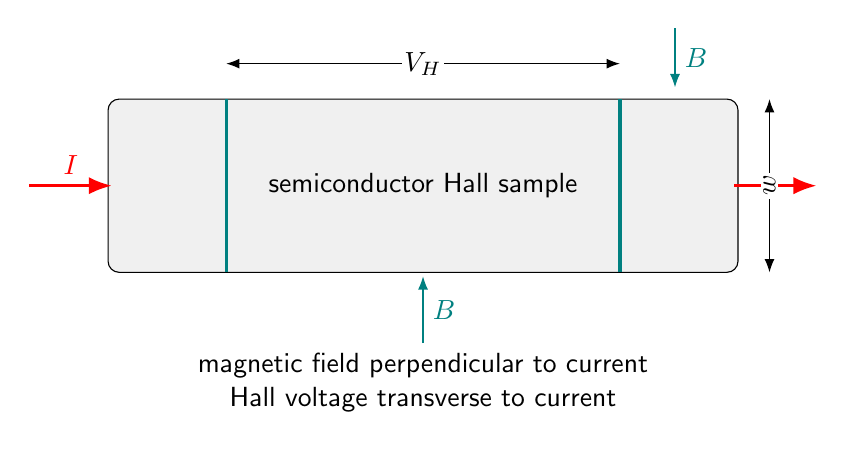
\begin{tikzpicture}[font=\sffamily,>=Latex]
\draw[fill=gray!12,rounded corners] (0,0) rectangle (8,2.2);
\node at (4,1.1) {semiconductor Hall sample};
\draw[red,very thick,-Latex] (-1,1.1)--(.05,1.1) node[midway,above] {$I$};
\draw[red,very thick,-Latex] (7.95,1.1)--(9,1.1);
\draw[teal,very thick] (1.5,0)--(1.5,2.2);
\draw[teal,very thick] (6.5,0)--(6.5,2.2);
\draw[teal,-Latex] (7.2,3.1)--node[right] {$B$}(7.2,2.35);
\draw[teal,-Latex] (4,-.9)--node[right] {$B$}(4,-.05);
\draw[<->] (1.5,2.65)--node[fill=white,inner sep=1pt] {$V_H$}(6.5,2.65);
\draw[<->] (8.4,0)--node[fill=white,inner sep=1pt,rotate=90] {$w$}(8.4,2.2);
\node[align=center] at (4,-1.4) {magnetic field perpendicular to current\\Hall voltage transverse to current};
\end{tikzpicture}
\end{document}
